\section{SEGUNDA SECCIÓN}

	\subsection{Resultados} \label{subsection:Resul_DFV}

Luego de aplicar el algoritmo mostrado en la \autoref{Cap4_Figura2} se obtuvieron las respuestas sísmicas de la edificación. 

\begin{figure}[!h]
     \centering
     \begin{subfigure}[b]{0.45\textwidth}
         \centering
         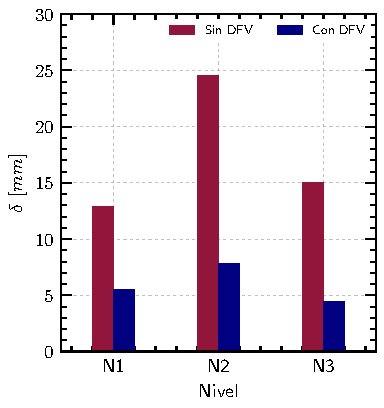
\includegraphics[scale=1]{E_IMAGENES/1_Capitulo4/Cap4_Imagen4a.pdf}
         \caption{\raggedleft Derivas de entrepiso $\delta$ \hspace*{0.5cm}}
         \label{Cap4_Figura4a}
     \end{subfigure}
	\hspace{3mm}
     \begin{subfigure}[b]{0.45\textwidth}
         \centering
         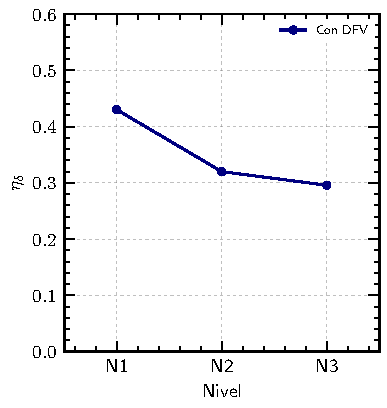
\includegraphics[scale=1]{E_IMAGENES/1_Capitulo4/Cap4_Imagen4b.pdf}
         \caption{\raggedleft Relación en derivas $\eta_{\delta}$ \hspace*{0.45cm}} 
         \label{Cap4_Figura4b}
     \end{subfigure}
        \caption[$\delta$ y $\eta_{\delta}$ en edificaciones con DFV]{\centering\footnotesize $\delta$ y $\eta_{\delta}$ en edificaciones con DFV.}
        \label{Cap4_Figura4}
     \vspace{5 mm}
	\end{figure}

	\begin{figure}[!h]
	\centering
		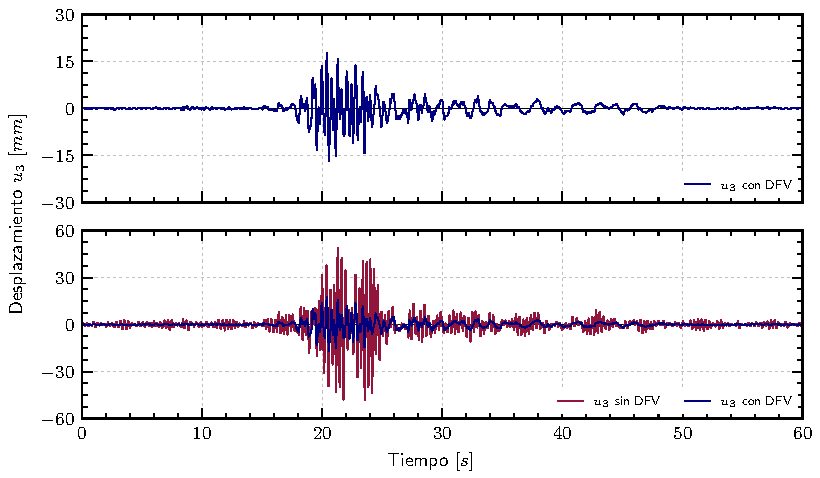
\includegraphics[scale=1]{E_IMAGENES/1_Capitulo4/Cap4_Imagen6.pdf}
		\vspace{-3 mm}
	\caption[Desplazamiento máximo del último nivel]{\centering\footnotesize Desplazamiento máximo del último nivel.}
	\label{Cap4_Figura5}
	\end{figure}


